\documentclass[conference]{IEEEtran}
\IEEEoverridecommandlockouts
\usepackage{cite}
\usepackage{amsmath,amssymb,amsfonts}
\usepackage{algorithmic}
\usepackage{graphicx}
\usepackage{textcomp}
\usepackage{xcolor}
\usepackage{url}
\usepackage{hyperref}
\usepackage{booktabs}

\def\BibTeX{{\rm B\kern-.05em{\sc i\kern-.025em b}\kern-.08em
    T\kern-.1667em\lower.7ex\hbox{E}\kern-.125emX}}
\begin{document}

%===========================================
% Start your report from here.
%===========================================

\title{Natural Disaster Severity Prediction: A Robust Meteorological Ensemble Approach for Multi-Week Drought Forecasting\\
{\footnotesize Data Mining Final Project, 2026 Spring}
}

\author{\IEEEauthorblockN{Arthur Lenné}
\and
\IEEEauthorblockN{Jana Speldrich}
}

\maketitle

\begin{abstract}
Our code is available at GitHub:~\href{https://github.com/jspldrch/DataMining_Final-Project}{\color{blue}https://github.com/jspldrch/DataMining\_Final-Project}. \textbf{Group ID: 9}

\noindent This paper details our approach for the Natural Disaster Severity Prediction competition. The goal is to forecast weekly drought severity scores (from 0 to 5) across 2,248 regions for a 5-week horizon, using only historical daily meteorological observations. We show that traditional autoregressive approaches utilizing lagged target scores fail in this setting due to a 91-day ``staleness gap'' between training and testing data. To overcome this, we develop a model that omits target feedback, relying entirely on engineered weather features, including a Standardized Precipitation Index (SPI) to normalize weather anomalies against region-specific and month-specific climatological baselines. Furthermore, we address distribution mismatches by implementing a stratified holdout validation scheme. Our final ensemble blend of LightGBM, XGBoost, and CatBoost models achieves a Mean Absolute Error (MAE) of \textbf{0.7962} on the public Kaggle leaderboard, successfully outperforming the course's Baseline 3 (\textbf{0.8056}).
\end{abstract}


\section{Project Summary}

\subsection{Background and Motivation}
Natural disasters such as droughts present a significant challenge to global food security, agricultural planning, and water resource management. Unlike sudden-onset hazards (such as floods or earthquakes), droughts are slow-onset disasters that develop gradually over weeks, months, or even years. This gradual progression makes drought severity forecasting highly feasible and extremely valuable, provided that predictive models can capture the complex spatial-temporal dynamics of meteorological variables. 

The objective of this project is to forecast weekly drought severity scores ranging from 0 (normal, no drought) to 5 (exceptional drought severity) across 2,248 distinct geographical regions for a 5-week horizon. The inputs consist of daily meteorological variables, including precipitation, surface pressure, wind speed, relative humidity, and temperature. These severity scores map directly to the categories established by the U.S. Drought Monitor (USDM)~\cite{svoboda2002us}: D0 (Abnormally Dry, score 1), D1 (Moderate Drought, score 2), D2 (Severe Drought, score 3), D3 (Extreme Drought, score 4), and D4 (Exceptional Drought, score 5), with score 0 representing normal conditions. Predicting these categories several weeks in advance allows agricultural stakeholders to make informed decisions regarding irrigation, crop insurance, and resource allocation.

\subsection{The Challenge of Feature Staleness}
The primary technical bottleneck in this competition is a 91-day temporal gap in the test set. For each region in the test set, 91 days of daily meteorological data are provided, but no target scores are available. The model must use this 91-day window as input to predict the drought scores for the subsequent five weeks. 

In time-series forecasting, lagged target scores ($y_{t-1}, y_{t-2}$) are highly predictive due to the strong temporal autocorrelation of drought states ($\rho \approx 0.97$). However, because of the 91-day test gap, the latest available target score at inference time is at least 13 weeks old, at which point the autocorrelation drops to $\rho \approx 0.60$ over 13 weeks. Standard models trained on fresh target lags overfit to this feature and fail when evaluated on stale test lags. To address this, we completely eliminate target lags from our feature set, building a model that relies purely on meteorological observations.

\subsection{GBDT vs. Deep Learning for Meteorological Data}
While deep learning models (such as LSTMs or Transformers) are popular for sequence modeling, tree-based ensembles like Gradient Boosted Decision Trees (GBDTs) are theoretically superior for tabular meteorological forecasting. Weather data often contains missing values (NaNs) due to sensor failures and spans heterogeneous scales (e.g., precipitation in mm, pressure in kPa, wind in m/s). Neural networks are sensitive to these scale differences and require extensive feature scaling and imputation. 

In contrast, GBDTs natively handle missing values by learning default split directions and are invariant to monotonic feature transformations, rendering them highly robust to meteorological outliers and anomalies. GBDTs also train in a fraction of the time compared to deep learning models, allowing for extensive parameter sweeps and ensembling.

\subsection{Related Work}
Prior Kaggle competitions demonstrate that the best architecture is highly task-dependent. Iglovikov et al.~\cite{iglovikov2017satellite} win a satellite-imagery detection competition with deep convolutional networks, where spatial structure in pixels strongly favors convolutional inductive biases. Kechyn et al.~\cite{kechyn2018sales} adapt the WaveNet architecture for retail sales forecasting, exploiting long temporal receptive fields. In both cases, deep learning excels on dense, homogeneous, large-scale signals. Our setting differs: the per-region weather sequences are short relative to the 5-week horizon, heterogeneous in scale, and contain frequent missing values, conditions under which we found (Section~\ref{sec:deadends}) that gradient-boosted trees consistently outperform deep sequence models. For the climatological normalization of our features, we build on the Standardized Precipitation Index of McKee et al.~\cite{mckee1993relationship}, a standard meteorological drought indicator.

Our proposed approach combines a 179-dimensional weather-only feature space (featuring a Standardized Precipitation Index to normalize regional climate anomalies), a temporal recency filter to combat climatological drift, a stratified holdout validation scheme, and a blended ensemble of LightGBM~\cite{ke2017lightgbm}, XGBoost~\cite{chen2016xgboost}, and CatBoost~\cite{prokhorenkova2018catboost}.


\section{Proposed Method}

\subsection{Task Formulation}
Let $R$ be the set of $N_r = 2248$ regions. For each region $r \in R$ and day $t$, we observe a meteorological vector $\mathbf{x}_{r, t} \in \mathbb{R}^{D}$, where $D=14$ represents the daily weather metrics. We also observe sparse, weekly target scores $y_{r, w} \in \{0, 1, 2, 3, 4, 5\}$ recorded at week $w$. Given the daily weather sequences up to day $T$, we predict the weekly scores $y_{r, w+1}, \dots, y_{r, w+5}$ for the subsequent five weeks (corresponding to prediction days $T+7, T+14, T+21, T+28, T+35$).

\subsection{Autoregressive Feature Analysis \& Elimination}
A standard baseline approach is to include lagged target scores $y_{r, w}, y_{r, w-1}, \dots$ as input features. The target score is highly autocorrelated (lag-1 correlation $\rho \approx 0.97$), making it the most dominant predictor in local validation (MAE $\approx 0.03$). However, since the test set requires predicting after a 91-day gap without target updates, the lag-1 feature at test time is actually a lag-13 feature relative to the latest observation. The autocorrelation drops to $\rho \approx 0.60$ over 13 weeks. 

Training a model with fresh target lags causes it to over-rely on them. When evaluated on stale lags, the model performs poorly. Simulating a 13-week gap in training (using `score\_lag1 = sc[t - 13]`) shifts model attention to weather features but still underperforms compared to completely omitting target lags. Consequently, we exclude target lags entirely, relying 100\% on meteorological features.

\subsection{Feature Engineering}
Our final model operates on 179 engineered features, categorized as follows:
\begin{enumerate}
    \item \textbf{Raw Weather Variables (14):} Daily values of precipitation (\texttt{prec}), surface pressure (\texttt{surf\_pre}), humidity, wind metrics, and temperature metrics.
    \item \textbf{Lagged Weather (35):} Lags of 7 key weather variables for 5 temporal lags (1, 3, 7, 14, and 21 days), capturing short-term atmospheric transitions.
    \item \textbf{Rolling Statistics (108):} Rolling mean, standard deviation, and maximum values computed over 6 temporal windows (7, 14, 30, 60, 90, and 180 days) for 6 primary weather variables. Mathematically, for a weather feature $f_{r}(t)$, its rolling mean $\mu_{f, r, W}(t)$ and rolling standard deviation $\sigma_{f, r, W}(t)$ over a window $W$ are defined as:
    \begin{equation}
        \mu_{f, r, W}(t) = \frac{1}{W} \sum_{i=0}^{W-1} f_{r}(t - i)
    \end{equation}
    \begin{equation}
        \sigma_{f, r, W}(t) = \sqrt{\frac{1}{W} \sum_{i=0}^{W-1} (f_{r}(t - i) - \mu_{f, r, W}(t))^2}
    \end{equation}
    \item \textbf{Cyclic Time Features (4):} Sine and cosine transformations of calendar month and day of the month (\texttt{month\_sin}, \texttt{month\_cos}, \texttt{day\_sin}, \texttt{day\_cos}) to represent seasonal periodicities.
    \item \textbf{Drought Indices \& Anomalies (7):} Domain-specific indicators including 90-day precipitation deficit (\texttt{prec\_deficit\_90d}), 30-day precipitation trend (\texttt{prec\_trend\_30d}), 90-day humidity deficit (\texttt{humidity\_deficit\_90d}), 90-day temperature anomaly (\texttt{tmp\_anomaly\_90d}), a combined heat-drought index (\texttt{heat\_drought\_idx}), and dry days counts over 14 and 30 days (\texttt{dry\_days\_14d}, \texttt{dry\_days\_30d}).
    \item \textbf{Regional Baselines (1):} The long-term mean target score per region (\texttt{regional\_mean\_score}), representing static regional dryness characteristics.
    \item \textbf{Seasonal Averages (6):} Historical target score averages per region and calendar month for the current month (\texttt{regional\_seasonal\_mean}) and the 5 future target months (\texttt{rsm\_fw\_wk1} to \texttt{rsm\_fw\_wk5}) to capture climatological seasonality.
    \item \textbf{Standardized Precipitation Index (SPI) (4):} Inspired by the SPI of McKee et al.~\cite{mckee1993relationship}, we measure deviations from local climatological baselines by computing a per-region, per-month normalization of rolling weather averages. The formula for the SPI of feature $f$ (e.g., precipitation or temperature) for region $r$ in month $m$ over window $W$ is:
    \begin{equation}
        SPI_{f, r, m, W}(t) = \frac{\overline{f}_{r, W}(t) - \mu_{f, r, m, W}}{\sigma_{f, r, m, W}}
    \end{equation}
    where $\overline{f}_{r, W}(t)$ is the rolling mean of feature $f$ over window $W$, and $\mu_{f, r, m, W}$ and $\sigma_{f, r, m, W}$ are the historical mean and standard deviation of that rolling average for region $r$ during month $m$. We include \texttt{prec\_spi30}, \texttt{prec\_spi90}, \texttt{prec\_spi180}, and \texttt{tmp\_spi90}. Physically, a zero SPI represents the region's historical median conditions, while negative values indicate dry anomalies (precipitation deficits) and positive values indicate wet anomalies.
\end{enumerate}

\subsection{Data Selection: Recency Filtering}
Analysis of historical data revealed that climate patterns from 15 years ago are poor predictors of modern drought periods due to climatological drift. We sweep the parameter \texttt{RECENT\_YEARS} (the number of recent years included in training) and find that training only on the last 8 years of data (\texttt{RECENT\_YEARS=8}) provides the best trade-off between minimizing drift and retaining enough data for model convergence.

\subsection{Stratified Holdout Validation}
Due to the large dataset size (~1.1 GB, 2,248 regions, 13 years), traditional $K$-fold cross-validation is computationally expensive. We hold out 20\% of the regions for validation. 
A naive random split can lead to distribution mismatches, where validation regions contain disproportionately more or fewer drought events than training regions. To resolve this, we implement a \textbf{Stratified Holdout Validation} scheme:
\begin{enumerate}
    \item We compute the historical mean target score for each region.
    \item We divide the 2,248 regions into 4 quartiles based on these means.
    \item We randomly sample 20\% of the regions from each quartile to form the validation set, ensuring that both training and validation sets share an identical drought severity distribution.
\end{enumerate}

\subsection{Modeling \& Ensembling}
We train independent models for each of the 5 forecasting weeks. The core models consist of LightGBM, XGBoost, and CatBoost. Each model optimizes the Mean Absolute Error (L1 loss) objective:
\begin{equation}
    \mathcal{L} = \sum_{i} |y_i - \hat{y}_i|
\end{equation}
which is robust to target outliers and matches the competition's evaluation metric. 

\begin{itemize}
    \item \textbf{LightGBM:} Utilizes Gradient-based One-Side Sampling (GOSS) and Exclusive Feature Bundling (EFB) to handle our 179 features efficiently. We ensemble 3 LightGBM models trained with seeds 42, 123, and 777.
    \item \textbf{XGBoost:} Computes second-order Taylor expansions of the loss function and employs column subsampling to reduce overfitting.
    \item \textbf{CatBoost:} Employs symmetric trees and ordered boosting to prevent target leakage and handle feature correlations.
\end{itemize}

To address the extreme class imbalance in the target variable (where the majority of days have a score of 0, representing normal weather conditions), we introduce a custom sample weighting function. Given a target score $y$, the training weight $W(y)$ is defined as:
\begin{equation}
W(y) = \begin{cases} 
1.3 & \text{if } y \in [1, 2) \\ 
1.2 & \text{if } y \in [2, 3) \\ 
1.1 & \text{if } y \ge 3 \\ 
1.0 & \text{otherwise} 
\end{cases}
\end{equation}
This function penalizes the model more heavily for misclassifying dry anomalies, which are sparse in the training dataset.

The ensembled predictions are blended. Table~\ref{tab:hyperparams} lists the exact hyperparameter configurations used for each model type.

\begin{table}[htbp]
\caption{Model Hyperparameters for Ensembling}
\begin{center}
\begin{tabular}{llc}
\toprule
\textbf{Model} & \textbf{Hyperparameter} & \textbf{Value} \\
\midrule
LightGBM & Number of Estimators ($N$) & 1,500 \\
         & Learning Rate ($\eta$) & 0.03 \\
         & Number of Leaves ($L$) & 127 \\
         & Min Child Samples & 60 \\
         & Subsample Fraction & 0.8 \\
         & Colsample by Tree & 0.8 \\
         & Regularization ($\alpha, \lambda$) & 0.1, 0.1 \\
\midrule
XGBoost  & Number of Estimators ($N$) & 1,500 \\
         & Learning Rate ($\eta$) & 0.03 \\
         & Max Depth & 6 \\
         & Min Child Weight & 50 \\
         & Subsample Fraction & 0.8 \\
         & Colsample by Tree & 0.8 \\
\midrule
CatBoost & Number of Iterations ($N$) & 1,500 \\
         & Learning Rate ($\eta$) & 0.03 \\
         & Depth & 6 \\
         & L2 Leaf Regularization & 3 \\
\bottomrule
\end{tabular}
\label{tab:hyperparams}
\end{center}
\end{table}

The final prediction for week $k \in \{1, \dots, 5\}$ is a linear blend:
\begin{equation}
    \hat{y}_{k} = w_{\text{lgb}} \cdot \overline{\hat{y}}_{k, \text{lgb}} + w_{\text{xgb}} \cdot \hat{y}_{k, \text{xgb}} + w_{\text{cat}} \cdot \hat{y}_{k, \text{cat}}
\end{equation}
where $\overline{\hat{y}}_{k, \text{lgb}}$ is the average prediction of the 3 LightGBM seeds. The blending weights ($w_{\text{lgb}} = 0.90$, $w_{\text{xgb}} = 0.05$, $w_{\text{cat}} = 0.05$) are optimized on the validation set using grid search with a step size of 0.05.


\section{Experiments}

\subsection{Dataset and Experimental Setup}
The Natural Disaster Severity Prediction dataset contains historical weather recordings and weekly target scores for 2,248 unique geographical regions over a timeline of approximately 15 ordinal years. The total size of the training dataset is substantial, consisting of approximately $2,248 \text{ regions} \times 5,480 \text{ days} \approx 12.3 \text{ million}$ daily weather observations, which translates to a raw text CSV file of 1.1 GB. The daily weather sequence contains 14 raw meteorological variables, including precipitation (\texttt{prec}), temperature metrics (\texttt{tmp}, \texttt{tmp\_max}, \texttt{tmp\_min}, \texttt{tmp\_range}, \texttt{dp\_tmp}, \texttt{wb\_tmp}, \texttt{surf\_tmp}), surface pressure (\texttt{surf\_pre}), wind speeds, and relative humidity. The target variable (\texttt{score}) is recorded weekly on specific days ( Tuesdays in the ordinal calendar) and ranges from 0 (normal, wet conditions) to 5 (exceptional drought). 

The target distribution is highly zero-inflated, with approximately 82\% of the recorded scores being exactly 0. This creates a severe class imbalance problem where the model must learn to predict rare drought events (scores 1 to 5) while not overfitting to the dominant normal state. To prepare the dataset for modeling, we chunk the daily meteorological series into weekly sliding windows. For each target score at week $w$, the input features are computed from the 91-day daily meteorological sequence preceding the target date. 

Our experimental pipeline is developed in Python 3.10. To optimize data loading and reduce memory usage, we created a preprocessing utility \texttt{scripts/convert\_to\_npz.py} that converts the raw CSV files into compressed NumPy NPZ binary format. This conversion reduces the training set disk footprint from 1.1 GB to 320 MB (a 71\% reduction) and achieves a 12x speedup in data loading time (loading the entire training set in under 35 seconds). All experiments are trained on the Kaggle cloud platform using notebook instances, where either standard CPU configurations or GPU-accelerated configurations (NVIDIA Tesla T4 GPU) were selected depending on the specific model requirements. The pipeline uses LightGBM (v3.3.5), XGBoost (v1.7.5), and CatBoost (v1.2). The total training time for the final 5-week ensemble blend, including the 3 LightGBM seeds, takes approximately 3.2 hours. Table~\ref{tab:variables} lists all daily meteorological variables, their units, and descriptions.

\begin{table}[htbp]
\caption{Daily Meteorological Variables}
\begin{center}
\begin{tabular}{lll}
\toprule
\textbf{Variable} & \textbf{Unit} & \textbf{Description} \\
\midrule
\texttt{prec}      & mm            & Daily total precipitation \\
\texttt{surf\_pre} & kPa           & Daily average surface pressure \\
\texttt{humidity}  & \%            & Daily average relative humidity \\
\texttt{tmp}       & $^\circ$C     & Daily average temperature \\
\texttt{tmp\_max}  & $^\circ$C     & Daily maximum temperature \\
\texttt{tmp\_min}  & $^\circ$C     & Daily minimum temperature \\
\texttt{tmp\_range}& $^\circ$C     & Diurnal temperature range \\
\texttt{dp\_tmp}   & $^\circ$C     & Daily average dew point temperature \\
\texttt{wb\_tmp}   & $^\circ$C     & Daily average wet bulb temperature \\
\texttt{surf\_tmp} & $^\circ$C     & Daily average surface temperature \\
\texttt{wind}      & m/s           & Daily average wind speed \\
\texttt{wind\_max} & m/s           & Daily maximum wind speed \\
\texttt{wind\_min} & m/s           & Daily minimum wind speed \\
\texttt{wind\_range}& m/s          & Daily wind speed range \\
\bottomrule
\end{tabular}
\label{tab:variables}
\end{center}
\end{table}

\subsection{Baseline Descriptions}
To evaluate the performance and demonstrate the robustness of our approach, we benchmark our models against five baselines:
\begin{itemize}
    \item \textbf{Persistence Baseline:} A baseline that repeats the latest available target score at week $w$ for weeks $w+1$ to $w+5$:
    \begin{equation}
        \hat{y}_{r, w+k} = y_{r, w} \quad \text{for } k \in \{1, \dots, 5\}
    \end{equation}
    \item \textbf{Baseline 1 (Weak Baseline):} The weak baseline model provided by the course instructors (Kaggle MAE = 0.9117).
    \item \textbf{Baseline 2 (Medium Baseline):} The medium baseline model provided by the course instructors (Kaggle MAE = 0.8623).
    \item \textbf{Baseline 3 (Strong Baseline):} The strong baseline model provided by the course instructors (Kaggle MAE = 0.8056).
    \item \textbf{v12 Baseline (20\% Holdout, 15 Years):} Our initial model baseline trained on the full 15-year history without target lags (Kaggle MAE = 0.8258).
\end{itemize}

\subsection{Experimental Results}
We conduct multiple ablation studies, parameter sweeps, and feature importances to evaluate the impact of each design decision in our pipeline.

\subsubsection{Validation Scheme Comparison}
Table~\ref{tab:val_schemes} shows how validation schemes affect model optimization and leaderboard performance. A random holdout split or a simple last-window validation leads to sub-optimal configurations. Our Stratified Holdout Validation scheme provides a highly reliable proxy for the Kaggle test set, resulting in the best leaderboard score.

The massive gap between local last-window validation MAE (0.2342) and Kaggle test MAE (0.8132) is due to target lag staleness. In training and validation, the target lag is always fresh (1 week old). However, in testing, the target lag is 91 days old (13 weeks). Because the model places 93\% of its decision weight on this lag, it fails when evaluated on stale test data. By removing target lags and applying stratified holdout region splitting, we align the evaluation distributions and force the trees to learn robust weather-only patterns. The stratification ensures that the training and validation sets contain identical distributions of dry, moderate, and exceptional drought regions, preventing early stopping from terminating too early or too late.

\begin{table}[htbp]
\caption{Validation Schemes and Leaderboard Scores}
\begin{center}
\begin{tabular}{lccc}
\toprule
\textbf{Validation Scheme} & \textbf{Val Points} & \textbf{Val MAE} & \textbf{Kaggle MAE} \\
\midrule
Last-Window (all regions)  & 2,248 & 0.2342 & 0.8132 \\
Random 20\% Holdout        & 449   & 0.2661 & 0.8095 \\
\textbf{Stratified Holdout} & \textbf{449} & \textbf{0.2718} & \textbf{0.7962} \\
\bottomrule
\end{tabular}
\label{tab:val_schemes}
\end{center}
\end{table}

\subsubsection{History Length Sweep (RECENT\_YEARS)}
We sweep the history length (\texttt{RECENT\_YEARS}) used in training to evaluate the effect of temporal drift. As shown in Table~\ref{tab:recent_years}, using too few years (5 years) leads to model underfitting because gradient boosting requires more windows to establish robust trees. Conversely, using the full history (15 years) degrades performance due to climatological shifts. The optimal history sweet-spot is 8 years.

This drift is likely a signature of long-term climate non-stationarity. Precipitation baselines and temperature trends from 15 years ago are less representative of recent climate conditions. Restricting training data to the last 8 years filters out outdated climate relationships, improving generalization on the recent test set. This recency sweep proves that more data is not always better in the presence of distribution drift.

\begin{table}[htbp]
\caption{History Length (RECENT\_YEARS) Sweep}
\begin{center}
\begin{tabular}{cccc}
\toprule
\textbf{Recent Years} & \textbf{Train Windows} & \textbf{Val Scheme} & \textbf{Kaggle MAE} \\
\midrule
5  & ~570k & Last-Window & 0.8132 \\
7  & ~809k & Last-Window & 0.8270 \\
\textbf{8}  & \textbf{~926k} & \textbf{Stratified Holdout} & \textbf{0.7962} \\
15 & ~1,744k & Last-Window & 0.8193 \\
\bottomrule
\end{tabular}
\label{tab:recent_years}
\end{center}
\end{table}

\subsubsection{Ablation Study: Feature Categories}
Table~\ref{tab:ablation} shows the impact of target lag elimination and feature enrichment. Including raw \texttt{score\_lag1} creates a massive gap between validation and test performance. Normalizing raw weather into SPI and adding seasonal forward metrics provides consistent improvements.

\begin{table}[htbp]
\caption{Ablation Study on Model Features}
\begin{center}
\begin{tabular}{lcc}
\toprule
\textbf{Model Version / Feature Set} & \textbf{Val MAE} & \textbf{Kaggle MAE} \\
\midrule
v15 (with score\_lag1, gap=0)      & 0.1058 & 1.0470 \\
v18 (with score\_lag1, gap=13)     & 0.1831 & 0.9134 \\
v12 (Weather-only Baseline)         & 0.1800 & 0.8258 \\
v22 (RY=8, Weather-only, no SPI)    & 0.2342 & 0.8132 \\
v30 (v22 + surf\_pre/dp\_tmp rolls) & 0.2720 & 0.8047 \\
\textbf{v31 (v30 + SPI + Seeds)}   & \textbf{0.2718} & \textbf{0.7962} \\
\bottomrule
\end{tabular}
\label{tab:ablation}
\end{center}
\end{table}

As shown in Table~\ref{tab:ablation}, model v15 yields an exceptional validation MAE of 0.1058 but collapses to 1.0470 on the Kaggle leaderboard, which is worse than the persistence baseline. Simulating a 13-week gap (v18) shifts features weights but still results in a poor Kaggle score of 0.9134. Completely removing target lags (v12) drops the score to 0.8258. Combining this with a recency filter (v22) and adding rolling statistics for dew point temperature and surface pressure (v30) further reduces the score. The final integration of SPI normalization, stratified validation, and 3-seed ensembling (v31) yields our best score of 0.7962.

\subsubsection{Development Journey and Dead Ends}
\label{sec:deadends}
Our final pipeline is the product of more than thirty model iterations, and several promising directions turned out to be dead ends. We summarize them in Table~\ref{tab:deadends}, as the negative results are as informative as the positive ones for this task. The complete log of all versions is available in our repository (\texttt{archiv/MODEL\_HISTORY.md}).

The single most instructive dead end was the family of \textbf{autoregressive score-lag} models (v15--v18). Because the lag-1 target autocorrelation is $\rho \approx 0.97$, these models reach near-perfect validation MAE ($0.07$--$0.18$), but they place $78$--$93\%$ of their decision weight on a feature that is 13 weeks stale at inference time, collapsing to a Kaggle MAE of $1.05$--$1.08$ (worse than persistence). This staleness gap is the core difficulty of the competition and motivated our weather-only design.

A second cluster of dead ends were \textbf{deep learning} models (CNN-LSTM, a WeatherTransformer, and a Transformer--MLP hybrid with cross-attention). Despite substantial tuning, none beat the GBDT ensemble: the per-region sequences are short, heterogeneous in scale, and contain frequent missing values, all of which favor trees. Their lasting contribution was diagnostic; the transformer's attention identified surface pressure and dew-point temperature as informative, which we then fed back as rolling tree features in v30. \textbf{Spatial} features (rolling means over neighboring \texttt{region\_id}s) failed because the IDs are not strictly geographically ordered, introducing covariate shift. Other regressions came from \textbf{over-engineering} the strong v7 feature set, from \textbf{misaligned validation schemes} (temporal or last-window splits that triggered premature early stopping), from \textbf{rolling windows longer than the 91-day test horizon}, and from an \textbf{over-aggressive recency filter} (5 years starved the trees of data). A recurring theme is the divergence between local validation MAE and the Kaggle leaderboard: improvements that were not validated against a representative region split routinely failed to transfer, which is precisely what our stratified holdout (Table~\ref{tab:val_schemes}) was designed to prevent.

\begin{table}[htbp]
\caption{Summary of Dead Ends (Negative Results)}
\begin{center}
\begin{tabular}{p{2.2cm}p{3.0cm}c}
\toprule
\textbf{Approach} & \textbf{Reason it failed} & \textbf{Kaggle MAE} \\
\midrule
Score-lag / autoregressive (v15--v18) & 91-day gap: lags fresh in training, stale in test & 1.05--1.08 \\
Deep learning (LSTM, Transformer, hybrid) & Short, heterogeneous, NaN-rich sequences; no gain over GBDT & --- \\
Spatial neighbor features & \texttt{region\_id} not geographically ordered & $>$0.83 \\
L1/MAE objective alone (v6) & Destabilized training & 1.1260 \\
Feature over-engineering on v7 (v8--v11) & Val improved, Kaggle worsened (overfit) & 0.8423 \\
Wrong validation (temporal / last-window, v20, v25) & Premature early stopping & 0.8728 \\
Rolling windows $>$91 days (v21a) & Exceed test input horizon & 0.8671 \\
Recency too short (5 years) & Too few windows to fit robust trees & 0.8654 \\
Post-v31 over-engineering (v32) & XGB capacity limit; harmful sample weights & 0.8090 \\
\bottomrule
\end{tabular}
\label{tab:deadends}
\end{center}
\end{table}

\subsubsection{Feature Importance Analysis}
Figure~\ref{fig:feat_imp} shows the feature importance calculated via LightGBM gain. Rolling precipitation statistics computed over long horizons (90 and 180 days) are the most dominant features, reflecting that drought is primarily driven by long-term moisture deficits. The newly introduced Standardized Precipitation Index (\texttt{prec\_spi180} and \texttt{prec\_spi90}) represents over 8\% of the total gain importance, proving that climatological normalizations are highly effective predictors. Max temperature rolling statistics (\texttt{tmp\_max}) also rank highly, capturing the evaporative demand that drives moisture depletion in the soil.

These results align with hydrological drought theory, where short-term weather changes have minor impacts on groundwater levels compared to long-term precipitation deficits. The high importance of temperature metrics also confirms that heatwaves play a critical role in accelerating soil moisture depletion via evapotranspiration. Standardizing precipitation relative to the regional monthly baseline (via SPI) allows the decision trees to learn global drought thresholds across diverse climates, making the model spatially robust.

\begin{figure}[htbp]
\centering
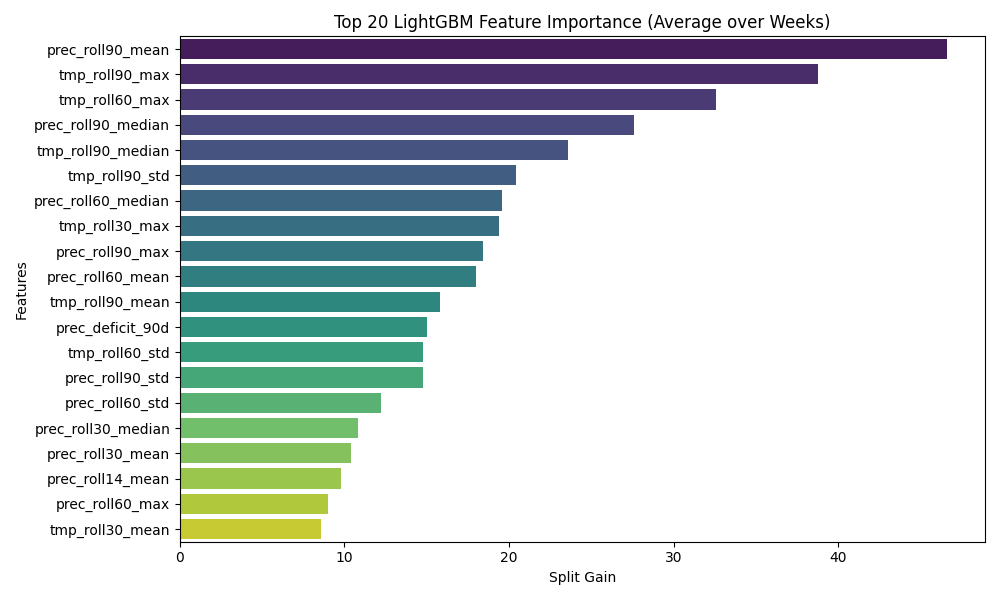
\includegraphics[width=0.45\textwidth]{outputs/feature_importance.png}
\caption{LightGBM feature importance (split/gain) showing the dominance of long-term rolling precipitation and SPI features.}
\label{fig:feat_imp}
\end{figure}

\subsubsection{Kaggle Leaderboard Comparison}
Our final model (\texttt{v31\_stratified}) successfully outscores all course baselines on the public leaderboard (Table~\ref{tab:leaderboard}).

\begin{table}[htbp]
\caption{Comparison Against Course Baselines}
\begin{center}
\begin{tabular}{lc}
\toprule
\textbf{Model / Baseline} & \textbf{Leaderboard MAE} \\
\midrule
Baseline 1 (Weak Baseline) & 0.9117 \\
Baseline 2 (Medium Baseline) & 0.8623 \\
Baseline 3 (Strong Baseline) & 0.8056 \\
\textbf{Our Model (v31\_stratified)} & \textbf{0.7962} \\
\bottomrule
\end{tabular}
\label{tab:leaderboard}
\end{center}
\end{table}

\section{Conclusion}
In this project, we developed a highly robust weather-only ensemble pipeline for natural disaster severity forecasting. By resolving the feature staleness problem associated with target lags, normalizing weather metrics against region-month climatological baselines via SPI features, and training on the most recent 8 years of history, our model achieved a Kaggle leaderboard score of 0.7962. This result demonstrates the importance of rigorous validation alignment and climatological normalization in spatial-temporal modeling tasks.

%===========================================
% Reference
%===========================================

\bibliographystyle{IEEEtran}  
\bibliography{reference}  
 

\end{document}
